\documentclass[11pt]{report} %size of font and type of layout
\usepackage[a4paper,margin=1in]{geometry}

\usepackage{pgfplots}
\usepackage{tikz}
\usepackage{xfrac}
\usepackage[super]{nth} %allow 1st, 2nd by typing \nth{1}, \nth{2}
\usepackage[title,titletoc,page]{appendix} %for using appendices
\usepackage{graphicx} %have images
\usepackage{chngcntr} %be able to make figures go 1, 2, 3 instead of 1.1, 1.2, 1.3, etc
\usepackage{subcaption} %have subfigures
\usepackage{wrapfig} %be able to wrap text around figures
\usepackage{amsmath} %a way to typeset maths
\usepackage{amssymb} %able to type maths symbols
\usepackage{textcomp} %so we can use \textdegree to get degree symbol
\usepackage[parfill]{parskip} %remove paragraph indentation
\usepackage{setspace} %be able to set line spacing
\usepackage{tocloft} %more control over table of contents, list of figures, etc
\usepackage{ltxtable} %get tabularx split over pages
\usepackage[english]{babel} %english-specific charaters and language rules
\usepackage{url} %type urls
\usepackage{parskip} %space between paragraphs
\usepackage[UKenglish]{isodate} %change date format
%\usepackage[hang,flushmargin]{footmisc} %no indents in footers
%\usepackage{verbatimbox} %able to use addvbuffer to change spaces before and after tables
\usepackage{pdfpages} %insert PDF pages
%\usepackage{titletoc} %create a small table of contents at the start of each section
\usepackage{microtype} %improves spacing between words and letters
\usepackage[nodayofweek]{datetime} %use \today to get the date
\usepackage[inline]{enumitem} %have inline lists
\usepackage{fancyhdr}		%for getting customized headers
\usepackage{lastpage}		%enable getting the total of the pages
%\usepackage{floatrow} %use for indicating figures' sources
%\usepackage{showframe} %show margins on page
\usepackage[hidelinks]{hyperref} %hyperlinks in pdf
\usepackage{cleveref} %automatic referencing
\usepackage{bookmark}
\DeclareGraphicsExtensions{.pdf,.png,.jpg,.eps} %can just give images' names
\usepackage{epstopdf} %allows for encapsulated postscript vector images, better quality and scalable
\usepackage[none]{hyphenat}		%kills all word breaks that were in annoying places

%--------------------------heading spacings----------------------------%
\usepackage{titlesec} %be able to change title settings
	\titleformat{\chapter}{\normalfont\huge\bfseries}{\thechapter.}{1em}{} %have number before chapter title
	\titlespacing{\chapter}{0pc}{0pc}{0pc} %have nice spacing after chapter title {indent} {before} {after}
	\titlespacing{\section}{0pc}{1pc}{0pc} %have nice spacing after section title {indent} {before} {after}
	\titlespacing{\subsection}{1pc}{1pc}{0pc} %have nice spacing after subsection title {indent} {before} {after}
	\titlespacing{\subsubsection}{0pc}{0pc}{-1pc} %have nice spacing after subsection title {indent} {before} {after}
	\titlelabel{\thetitle.\quad} %full stop after the number in the heading title
\usepackage{etoolbox} %remove page break before chapter heading
	\makeatletter
	\patchcmd{\chapter}{\thispagestyle{plain}}{\thispagestyle{fancy}}{}{} %allows the header/footer on chapter pages
	\patchcmd{\chapter}{\if@openright\cleardoublepage\else\clearpage\fi}{}{}{}
	\makeatother
%----------------------------figures & lof (list of figures)-----------------------------%
\renewcommand{\cftfigfont}{Figure } %list of figures includes "Figure"
\newcommand*{\noaddvspace}{\renewcommand*{\addvspace}[1]{}}\addtocontents{lof}{\protect\noaddvspace} %equal line spacing in the list of figures
\setlength{\cftfigindent}{0pt} %remove indentation from figures in lof
\usepackage{float} %able to use H to force figures to go here
%\floatstyle{boxed}	%this will place a thin border around my figures
%\restylefloat{figure}
\AtBeginEnvironment{figure}{\vspace{10pt}} %spacing before figure
\AtEndEnvironment{figure}{\vspace{-10pt}} %spacing after figure
\setlength{\abovecaptionskip}{10pt} %spacing before figure caption
\setlength{\belowcaptionskip}{5pt} %spacing after figure caption
\usepackage[justification=centering,font={normalsize, it}]{caption} %control caption text
%----------------------------tables & lot------------------------------%
\renewcommand{\cfttabfont}{Table } %list of tables includes "Table"
\setlength{\cfttabindent}{0pt} %remove indentation from tables in lot
\usepackage{tabularx} %word wrap in tables
\usepackage{longtable} %allow tables to go over multiple pages
\usepackage{multirow} %make cells span multiple rows in tables
\captionsetup{belowskip=5pt,aboveskip=4pt}
\newcolumntype{L}{>{\centering\arraybackslash}m{3cm}} %centre and wrap text in tables
\usepackage{booktabs} %use \toprule, \midrule, \bottomrule and \cmidrule for better spacing in tables
\usepackage{pbox} %force line break in a table cell
%---------------------------create own lists---------------------------%
\newlistof{example}{exp}{List of Examples} %create own lists
\newcommand{\example}[1]{ %create own lists
	\refstepcounter{example} %create own lists
	\par\noindent\textbf{Example \theexample. #1} %create own lists
	\addcontentsline{exp}{example} %create own lists
	{\protect\numberline{\thechapter.\theexample}#1}\par} %create own lists
%---------------------------------font---------------------------------%
%\sfdefault = calibri-like font, \rmdefault = times new roman-like
\renewcommand\UrlFont{\rmfamily}
\renewcommand{\familydefault}{\rmdefault}
%----------------------------------------------------------------------%
\begin{document}
\begin{onehalfspace} %single line spacing
%\counterwithout{figure}{chapter} %makes figures go 1, 2, 3 instead of 1.1, 1.2, 1.3, etc
%\counterwithout{table}{chapter} %makes tables go 1, 2, 3 instead of 1.1, 1.2, 1.3, etc
%\counterwithout{section}{chapter} %make sections 1, 2, 3 not 1.1 etc
\pretolerance=10000 %disable hyphenating at line breaks
\abovedisplayskip=5pt %remove space before equations
\belowdisplayskip=5pt %remove space after equations
\cleanlookdateon %remove current date format to replace with [UKenglish]{isodate}
%\let\savenumberline\numberline\def\numberline#1{\savenumberline{#1.}} %adds dot after chapter title in toc, comment this out to get appendices to work and not cause spacing errors.
\AtEndEnvironment{itemize}{\vspace{-5pt}} %spacing after lists 

\newcommand{\thetitle}	{Business Plan}
\newcommand{\theauthor}	{Roberto Aldera - ALDROB001 \\ Gareth Callanan - CLLGAR010 \\ Luke Goemans - GMNLUK001 \\ Benjamin Scholtz - SCHBEN011 \\ Munawwar Tayob - TYBMUN001 }
\newcommand{\studentnum}{}
\newcommand{\thedate}	{\today}
\newcommand{\coursecode}{EEE4051F}
\newcommand{\coursename}{New Venture Planning}
\newcommand{\staffmember}{Dr. Peter Martinez}

\pagenumbering{gobble}	%no page number for title page
\renewcommand\headrulewidth{0pt}	%get rid of stray header underline
	\begin{center}
\begin{minipage}{1\textwidth}
\begin{center}
	
\begin{center}
\includegraphics[width=1\linewidth]{"UCThoriz"}
\end{center}
\vskip20pt
\Large{Faculty of Engineering and the Built Environment}\\
Department of Electrical Engineering\\
\coursecode
\vskip10pt
\begin{figure}[H]
\centering
\hspace{-3em}
\includegraphics[width=0.6\textwidth]{images/uvuka_logo_ben}
\vskip20pt
\end{figure}
\hrule
\vskip20pt
\Huge\sc{\thetitle}
\vskip20pt
\hrule
\vskip20pt
\Large\textnormal{\textbf{Team 5:}\\
\theauthor\\
\vskip10pt
\textbf{Lecturer:} \staffmember
\vskip20pt
\hrule
\vskip20pt
\thedate\\}
%\textbf{\assignmentname}
\end{center}
\end{minipage}
\end{center}

\newpage 	
%	\chapter*{Plagiarism Declaration}
We know that plagiarism is wrong. Plagiarism is to use another's work and pretend that it is our own.

We have used the IEEE convention for citation and referencing. In this report, all contributions to, and quotations from, the work(s) of other people have been cited and referenced. 

This report is our own work. We have not allowed, and will not allow, anyone to copy our work.
\vskip100pt
\begin{center}
	Signed: \line(1,0){200}
	\vskip20pt
	Dated: \line(1,0){200}
\end{center}

\newpage
%	\renewcommand{\contentsname}{Table of Contents} %change table of contents's name from 'contents' to 'table of contents'
\newpage %page break
\phantomsection %for some reason this gets the bookmarks to work

\tableofcontents



%\addcontentsline{toc}{chapter}{Section:} %add "table of contents" to the table of contents
\newpage %page break
\renewcommand\headrulewidth{0.4pt}

\pagenumbering{roman}	%start the page numbering (and reset it to zero)
\pagestyle{fancy}
\fancyhf{}
\rhead{Group 5}
\lhead{\coursecode \\ \coursename}
\cfoot{\thepage}

\newpage
\chapter*{Executive Summary}
\addcontentsline{toc}{chapter}{Executive Summary}
Write this last.
\section*{Problem background}

\section*{Product description}

\section*{Marketing strategy}

\section*{Financial projections}

\section*{Anything else? Help...}


\cleardoublepage
\phantomsection
\addcontentsline{toc}{chapter}{Table of Contents}
\renewcommand{\contentsname}{Table of Contents} %change table of contents's name from 'contents' to 'table of contents'
\newpage %page break
\phantomsection %for some reason this gets the bookmarks to work

\tableofcontents



%\addcontentsline{toc}{chapter}{Section:} %add "table of contents" to the table of contents
\newpage %page break
\newpage

\cleardoublepage
\phantomsection
\addcontentsline{toc}{chapter}{List of Figures}
\listoffigures
\newpage

\pagenumbering{arabic}	%start the page numbering (and reset it to zero)
\chapter{Introduction}
In South Africa, there were 4500 road accidents which claimed the lives of more than 5500 people between 2014 and 2015 \cite{EWNRoadDeaths}. **The identified problem can be expanded here

Uvuka seeks to reduce the number of deaths on the road by providing a driver-monitoring device, which will set off alarms when a driver becomes drowsy and closes their eyes. This device is targeted at drivers who spend lots of time on the road and are prone to fatigue. It can be used by individuals or by companies who own fleets of trucks, buses, or taxis. The device is powered via the 12V DC electrical system in the car and is activated when the driver turns on the ignition switch. A camera is mounted on a vehicle's dashboard which faces the driver, and uses image processing algorithms to detect the frequency of blinking. If the driver is believed to be falling asleep or if a face is not recognized (the driver is not facing the road), a warning sound is emitted from the device to wake up the driver. 

Uvuka has thus developed a flexible product which can be uniquely designed for the following target markets in South Africa:
•	Freight Industry 
•	Public Transport
•	Private





As we are a growing company, we will need some capital investments in order to get our products to market. In return for an investment of R400 000 for (40\% or 20\%) of the company’s shares in year 1, investors can expect to receive dividends in the 3rd year of operation, and after 5 years receive cumulatively R600 000 NPV in dividends.

Uvuka has developed its first product, Uvuka Pro, which is specifically designed for transport companies which manage a fleet of vehicles. This device will be permanently mounted inside the companies vehicles and will be linked to the companies main control room. In this way, the company will be made aware of audio warnings given to the drivers of the vehicles. If the driver receives an ongoing warning sound, in the case that their eyes have been closed for too long a period, then the control center is alerted so that they can make radio contact with the driver and ensure their safety. 
How will it alleviate/solve/increase/decrease here



possible points to consider in intro?\\
- other companies trying to provide solution to this need \\
- before technology not available or cheap enough to implement \\
- product keeps drivers awake when they become drowsy \\
- 

\newpage
\chapter{Product Description}
\section{Product Overview}
Uvuka seeks to reduce road accidents through intelligent monitoring of vehicle drivers. The product consists of a single device that mounts onto the dashboard of a vehicle, as seen in \cref{fig:Uvuka_casing_concept}. The basic working version of the product will have a camera pointing in the direction of the driver that focuses on the driver's eyes. The device will monitor a driver's eyes and detect if they close. If the eyes close for a set period of time (longer than the average blink), then the device assumes that the driver is sleeping and takes corrective measures to wake the driver up.

\begin{figure}[H]
\centering
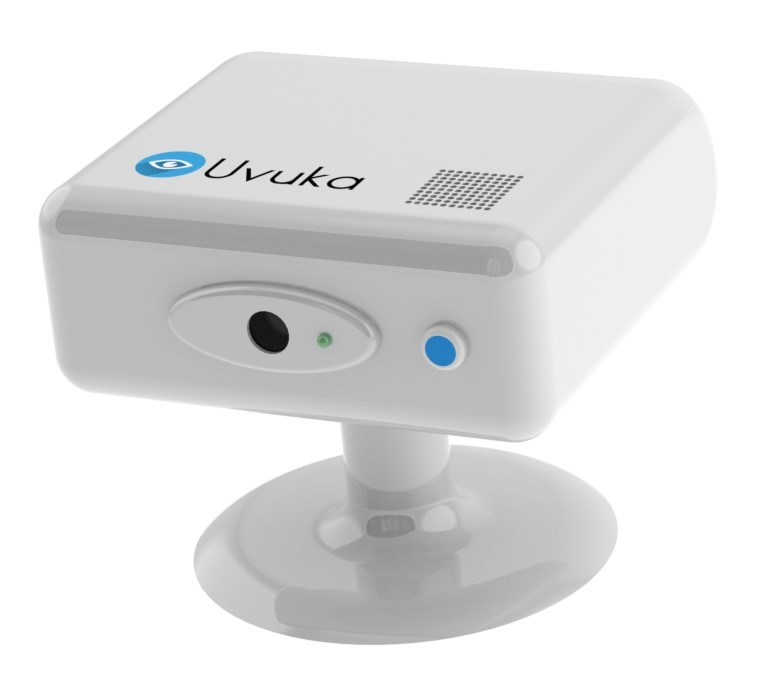
\includegraphics[width=0.6\textwidth]{images/Uvuka_casing_concept.JPG}
\vskip10pt
\caption{Conceptual design of Uvuka device rendered in SolidWorks}
\label{fig:Uvuka_casing_concept}
\end{figure}

Uvuka consists of a range of products. This product range will all center around the same goal (keeping the driver awake) but with different features present in different models. The first prototype produced will be the most elementary device, and once orders have been secured and units delivered,  more complex products can be developed and sold.

\section{Technical description of Uvuka}
\label{sec:Technical description of Uvuka}
The basic product consists of four main hardware components:
\begin{enumerate}
  \item \textit{Cabin Camera} - The cabin camera faces the driver and provides a real-time video feed of their face, upon which algorithms can be performed. The camera is able to capture suitable low light footage for all driving conditions.
  \item \textit{Audio Speaker} - The audio speaker is used to alert the driver. The speaker will play randomly generated tones that vary in frequency and duration. This prevents the driver from growing accustomed to the tones and thus will be more likely to wake him up \cite{Habituation}.
  \item \textit{Micro-controller and Inertial Navigation System} - The micro-controller needs to be powerful enough in order to perform real-time video processing. Eye-tracking and detection is done using OpenCV algorithms - these are free and open source video and image processing software algorithms. The micro-controller will also control the speaker and begin to play sounds when the driver begins to fall asleep \cite{OpenCV}. An Inertial Navigation System (INS) will include the necessary accelerometers, gyroscopes, and magnetometers to record the vehicle's dynamics and driver's handling of the vehicle.
  \item \textit{Power Supply} - The device can either be plugged into the standard 12 V cigarette plug, or it can be directly connected to the car power source for permanent mounts. The power is regulated to the correct voltage within the device, which will also include surge protection.
\end{enumerate}

The product has various modes of operation as seen in \cref{fig:DeviceFlowChart} below. The system defaults to the passive scanning mode where the device detects the driver's face and monitors eye movement. If the eye is determined to be closed, the device  enters a minor emergency state and assumes the driver's concentration has begun to wane. A brief sound is emitted to alert the driver. If this does not cause a satisfactory level of alertness, it assumes the driver is at risk of falling asleep and proceeds to take more drastic action. The action taken depends on the time the driver remains unresponsive and will vary from one type of device to the other.

\begin{figure}[H]
\centering
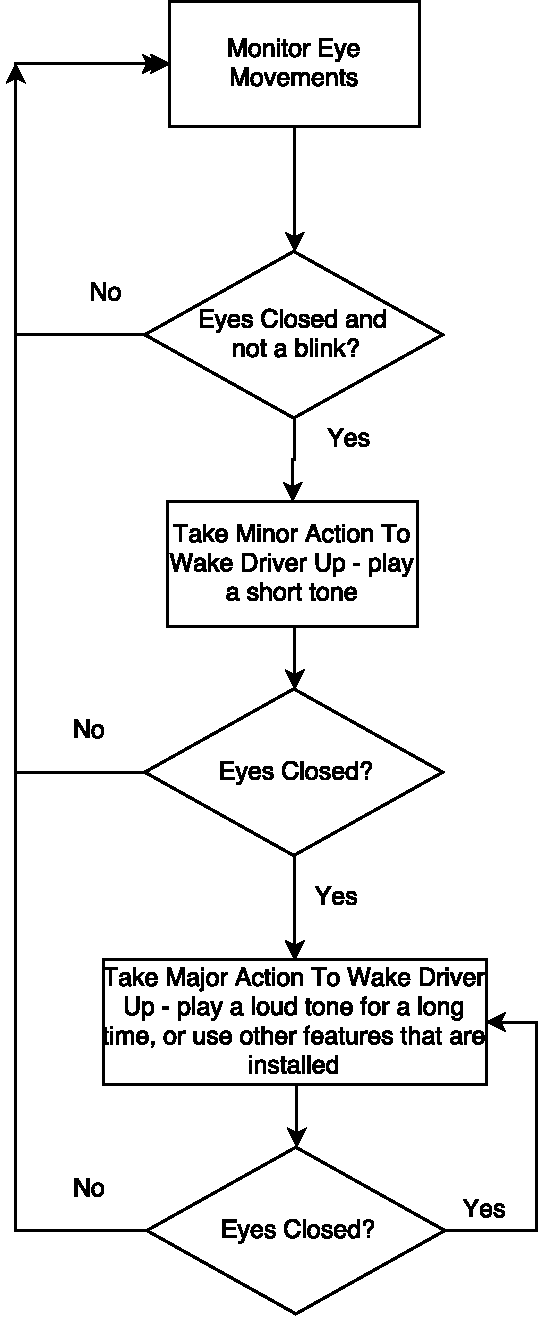
\includegraphics[width=0.4\textwidth]{images/ProductFlowchart}
\vskip10pt
\caption[Device Operation Activity Diagram]{Activity Diagram of the device operation}
\label{fig:DeviceFlowChart}
\end{figure}

\section{Product Range}
The the device prototype explained in \cref{sec:Technical description of Uvuka} above is envisioned as being the entry level product that private consumers will be able to purchase. This will be targeted for those on a tighter budget who require this device. As the business grows, the product range will be expanded based on consumer feedback and market research.

There are a number of other products and expansions planned:
\begin{itemize}
\item Frequent Driver Uvuka camera - This product is aimed at taxi operators and delivery drivers that are behind the wheel for extended periods of time. They are more likely to drive while tired or near exhausted (some taxi drivers can have shifts over 14 hours long \cite{taxiDriverHours}). In this case, sound may not be enough to wake them up. This product will have a strip attached to the steering wheel that will vibrate if the driver begins to fall asleep.
\item Long Distance Transport Uvuka camera - this product also incorporates the cabin camera and vibrating steering wheel attachment. Additionally, it also has a second camera facing the road in front of the driver and a GPS unit to track the vehicle's location. All this data is recorded on an SD card. This system is aimed for long distance freight vehicles and allows fleet managers to monitor their drivers and vehicles through the INS data for quality and insurance purposes.
\end{itemize}

\section{Competitor product analysis}
There are currently two primary international competitors producing a similar product. Seeing Machines, a company based in Australia, have developed a technology that tracks driver eyelid movement through computer vision algorithms \cite{SeeingMachinesWebsite}. They monitor the frequency and duration of blinking, as well as eyelid velocity. If the driver’s head begins to drop, an audio alarm is triggered and the seat vibrates. If they fall asleep again, a dispatcher is alerted and may make radio contact with the driver to check if they need a break. Seeing Machines has specifically worked with drivers that operate Caterpillar mining equipment \cite{SeeingMachinesWired}.

The second competitor company is Exeros, based in the United Kingdom \cite{Exeros}. Their product is targeted at businesses that operate a fleet of vehicles. When the driver begins to fall asleep, audio tones are sounded to attempt to wake them up. The devices they produce are able to be connected to an external GPS so that when an alarm is triggered, an outside individual can be notified of the occurrence and the location.

% --Extra sources/info--
% Toyota has implemented a driver alertness sensor as early as 2008 in their upmarket Toyota Crown cars. This camera detects the upper and lower eyelids, calculating how open they are. The car has built-in proximity sensors outside the car to measure what’s happening and to apply the brakes or prepare the airbags depending on the probability of a collision.

% HARMAN technology has developed a pupil-based driver monitoring system which interprets the level of the driver’s cognitive load and mental multitasking ability, adapting the car’s interface and connected devices accordingly. This drowsiness monitoring can cause the car to automatically turn the driver’s mobile device into do-not-disturb mode or adjusting ADAS system intervention thresholds to minimize physical and mental distraction to the driver.
% IQ Intel

\section{Advantages of Uvuka over competitor products} 
Uvuka’s unique features allow it to perform several of the tasks currently performed by competing products.
%TODO expand on this section^^^

\section{Product positioning}
The product will be versatile enough to cater for the needs of a number of industries. The following sectors are considered:
\begin{itemize}
\item Heavy duty freight truck drivers
\item Bus drivers
\item Construction equipment operators (cranes, diggers, etc.)
\item Taxi drivers
\item Private use
\end{itemize}

\section{Intellectual Property and freedom of trade}
%Luke wants to do this section :P

\newpage
\chapter{Marketing Plan}
\section{Problem background}
Over 5500 people lost their lives in 4500 accidents on South Africa's roads between 2014 and 2015. This harrowing statistic motivated the company to engineer a product capable of making our roads a safer place for all \cite{EWNRoadDeaths}. 

South Africa's railway system is currently unable to support the needs of the growing economy. With 88\% of all freight being moved on the roads \cite{BDlive_freight}, many truck drivers are exposed daily to the risks of falling asleep at the wheel \cite{ArriveAliveDriverTiredness} and increase the risk of road accidents caused by fatigue \cite{News24TruckersSleeping}.

In addition, \cref{tab:deaths100thousand} shows that South Africa is significantly behind both developed and developing countries in the effort to curb road accident deaths, ranked \nth{36} in the world for number of road deaths per 100 000 inhabitants \cite{deathsPer100thousandStats}.


\begin{table}[htbp]
  \centering
  \caption{Indication of South Africa's road death crisis}
    \begin{tabular}{cc}
    \toprule
    \textbf{Region} & \textbf{Road deaths per 100 000 inhabitants} \\
    \midrule
    South Africa & 27.6 \\
    North America & 10.4 \\
    Australia & 5.6 \\
    Argentina & 12.0 \\
    Colombia & 12.0 \\
    Malaysia & 23.8 \\
    \bottomrule
    \end{tabular}%
  \label{tab:deaths100thousand}%
\end{table}%

To understand the regional road death statistics, the figures over the two-month festive season 2014/2015 in which 1 376 fatalities occurred are shown in \cref{fig:festiveSeason}. Each province experiences varying fatalities depending on its size and population density \cite{ProvincialFestiveStats}. Most notably, Gauteng and KwaZulu-Natal make up for a significant portion of the fatalities with 223 and 237 deaths respectively. Uvuka will seek to target customers operating in these two provinces specifically by setting up head offices in Johannesburg.

\begin{figure}[H]
\centering
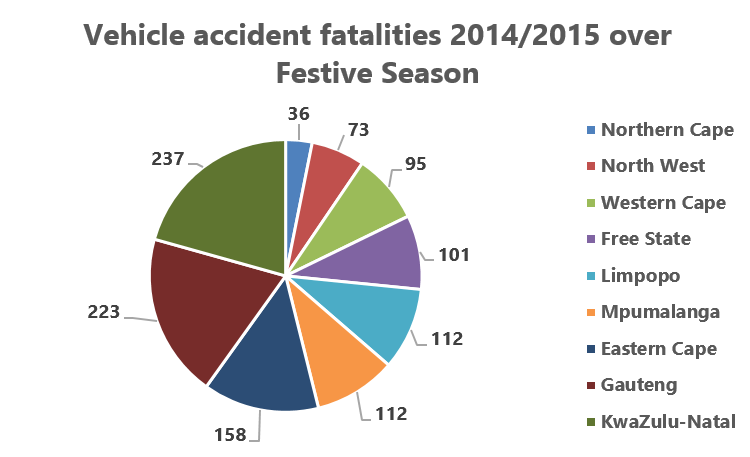
\includegraphics[width=0.8\textwidth]{images/provincial_fatalities.PNG}
\vskip10pt
\caption[Provincial fatalities for the period from 1 December 2014 to 7 January 2015]{Provincial fatalities for the period from 1 December 2014 to 7 January 2015}
\label{fig:festiveSeason}
\end{figure}

\section{Market strategy}
Once the context in which the device will operate is established, a market analysis will provide improved targeting of potential customers and insight into market trends. No South African competitors currently exist and so the company is expected to capture a significant portion of the market due to the product’s relative novelty and necessity.

\subsection{Initial market research}
Approximately three months will be set aside once the business has begun in order to conduct extensive research into the current market for this product. This will allow for better product positioning and ensure maximum impact of any targeted advertising. The following areas will need to be investigated:
\begin{itemize}
	\item \textit{How much will an Uvuka device cost to manufacture?} - manufacturing companies will need to be contacted before the prototyping process in order to accurately estimate the costs involved.
	\item \textit{What are customers prepared to pay for a driver monitoring device?} - truck companies and commercial drivers will be asked what their expectations are for the products features and its price.
	\item \textit{How many Uvuka devices will be required in order to curb road accident deaths in South Africa?} - South African road accident statistics will need to be further analysed in order to provide a reasonably accurate estimate of this figure.
	\item \textit{Which companies should the business approach for the first stage of product roll-out?} - an investigation into which companies travel in the more dangerous provinces will provide further insight.
	\item \textit{How will commercial drivers react to being monitored constantly?} - drivers will need to be interviewed in order to obtain their feedback. This way Uvuka will be able to position itself as a tool that saves lives, and not something that is there to spy on employees.
\end{itemize}

 \subsection{SWOT analysis}
A SWOT analysis is a common market research tool that analyses the Strengths, Weaknesses, Opportunities and Threats faced by a particular company. This is presented in \cref{tab:SWOT} below:
% Table generated by Excel2LaTeX from sheet 'Sheet1'
\begin{table}[htbp]
	\centering
	\caption{SWOT analysis of Uvuka}
	\begin{tabular}{|m{3cm}|m{6cm}|m{6cm}|}
		\hline
		\textbf{SWOT:} & \textbf{Helpful} & \textbf{Harmful} \\
		\hline
		\textbf{Internal origin} & \textbf{Strengths:}  compact size, realtively low-cost, multifunctional (GPS, sensors, camera, alerts), outsourced manufacturing of components with insourced assembly to control quality, initial small-scale enables rapid adjustments and fine tuning, low power consumption, potential to add a road-monitoring camera for insurance purposes in the second phase of products & \textbf{Weaknesses:} people often dislike being monitored, the device may be seen as an intrusion, devices are at risk of being tampered with, success relies on established companies to try something new from a small start-up (reluctant customers), legal implications if vehicle crashes due to driver fatigue despite Uvuka monitoring being installed \\
		\hline
		\textbf{External origin} & \textbf{Opportunities:} no immediate local competitors, the market could be dominated quickly, growing economy requires more trucks on the road, companies are looking to keep their drivers and loads safer, government is constantly seeking to reduce death toll on roads & \textbf{Threats:} devices may be easy to replicate and so new competition could catch up quickly, employers could misuse devices to spy on employees, risk of theft as device is very visibly mounted onto dashboard \\
		\hline
	\end{tabular}%
	\label{tab:SWOT}%
\end{table}%

\section{Uvuka product name and logo}
``Uvuka" literally means ``wake up" in Zulu. Other variations of the word are ``vuka" (get up) or ``uvukile" (to wake up), but it was felt that ``Uvuka" was the most suitable of these derivatives. This name gives an indication of the urgency in waking up, as well as a direct link to the South African origins of the company.

In order to convey the product's purpose and the company's values, a logo was designed as seen in \cref{fig:uvuka_logo}. This seeks to motivate the product to potential investors and customers as a device that keeps an eye open in order to ensure your safety or the safety of your employees on the roads.

\begin{figure}[H]
\centering
\includegraphics[width=0.7\textwidth]{images/uvuka_logo_ben}
\vskip10pt
\caption[The Uvuka logo]{The Uvuka logo}
\label{fig:uvuka_logo}
\end{figure}

\section{Strategic partnerships}
In order to gain more traction in the market, Uvuka will seek to partner with the Automobile Association (AA) in South Africa. This will allow us to gain accreditation and influence within the automotive sector which is always seeking new ways to improve safety on the nation's roads.

In addition to the AA, a partnership with an insurance company like Santam or Mutual \& Federal would be beneficial. Our devices would be able to reduce the insurance risk on the road and allow the insurer to offer a lower premium on their clients' policies that cover vehicles fitted with Uvuka hardware.

\newpage

\chapter{Finances}

Money money money, Moooooooney: https://www.youtube.com/watch?v=f9zraS8EKw4 

Its a rich man's world: https://www.youtube.com/watch?v=ETxmCCsMoD0

\section{Time-line of Operation}
In order to accurately estimate the finances of the company, a time-line of how the business operations is constructed:

{\bfseries 1st Quarter of Operations}
\begin{itemize}
\item An initial amount of R250 000 is injected by the owners into the business.
\item All five owners start working at the same time for a salary of R10 000 a month each.
\item All owners are working out of their private residences for the first quarter and as such no rent needs to be paid.
\item The prototyping stage begins. This R50 000 is used to buy and manufacture the components
\item R20 000 is used to purchase a high end desktop PC to run simulations as well as a printer.
\end{itemize}

{\bfseries 2nd Quarter of Operations}
\begin{itemize}
\item R500 000 is invested into the company by external investors
\item Office space is rented for approximately R14 000 a month.
\item Prototyping is completed after the fifth month.
\item Products are manufactured and sold in the sixth month of operation.
\end{itemize}

{\bfseries 3rd Quarter of Operations}
\begin{itemize}
\item A salesperson is hired at the start of the third quarter for R10000 a month.
\end{itemize}

{\bfseries 4th Quarter of Operations}
\begin{itemize}
\item The fourth quarter is used to do more market research and locate potential clients. No new operating expenses are incurred here.
\end{itemize}

{\bfseries 2nd Year of Operations}
\begin{itemize}
\item Manufacturing is increased in the second year. A loan of R500 000 is taken out from a bank at an interest rate of 10\% to be paid over ten years. 
\item A technician is hired for R10000 an month salary.
\item The 5 original owners have their salary increased to R11000 a month.
\item A part time cleaner is hired to clean the office for R5000 a month
\end{itemize}

{\bfseries 3rd Year of Operations}
\begin{itemize}
\item Product starts being marketed to the general public. This does not mean direct sales to freight companies are stopped, the target market is just expanded. Advertising is taken out to market it.
\item Owners have their salary increased to R13 000 a month.
\end{itemize}

{\bfseries 4th Year of Operations}
\begin{itemize}
\item One more technician is recruited. The new recruits salary matches the other employees salaries.
\item All staff members receive a salary increase of 6\%.
\end{itemize}

{\bfseries 5th Year of Operations}
\begin{itemize}
\item The business is on track to reach a yearly turnover of R5 Million by the end of this year. Options will be explored to manufacture products in house.
\end{itemize}

There are some other costs that will be included in the expenses:
\begin{itemize}
\item Office supplies
\item Insurance - the cost of risk insurance will be determined when the product has been manufactured.
\end{itemize}

%TODO product markup section
\section{Expected Product Cost and Markup}   

Estimations for the amount of products produced and sold are made in \cref{tab:tblProductSales}. Very few products are produced in the first year of operation as a portion of the year is spent developing the product and making an initial entry into the market. The final product is the largest expense by far for the business. This table assumes that when additional products are released they will cost as much as the basic version. This is therefore a conservative estimate as later additions could potentially be sold at a higher markup while still costing about the same amount to manufacture. The values listed are excluding VAT which must be included when selling to the vendor. The cost to assemble the raw materials and have them manufactured is shown in the appendix in \cref{tab:productCost}. The total cost of product is worked out using the raw material and manufacturing costs but also included the labour costs(technicians salaries). This priced is increased every year according to inflation. 

%The filled in table can be found in the cashflow.xls file in the drive
%TODO fill in this table correctly
\begin{table}[htbp]
  \centering
  \caption{Table showing the estimated income and costs for manufacturing the product}
    \begin{tabular}{rrrrr}
    \toprule
    Year of Operation & Quantity Produced& Quantity Sold& Cost Price & Selling Price \\
    \midrule
    1     &       &       &  	&\\
    2     &       &       &  	&\\
    3     &       &       &  	&\\
    4     &       &       &  	&\\
    5     &       &       &  	&\\
    Total     &       &       &  	&\\
    \bottomrule
    \end{tabular}%
  \label{tab:tblProductSales}%
\end{table}%


%TODO tax section
\section{Tax}

An unfortunately unavoidable  expense is tax. In the cash flow statement, the flow of money into the business is taken as the selling price after tax has been discounted. The next  


\section{Employee Cost Breakdown}

Salaries are the second highest cost for the business. The salary breakdown is shown in \cref{tab:salaries}. The founders start off with a very low salary but this will increase greatly as the profitability of the business increases. Only a single salesperson is needed as it is assumed the founders will also take part in selling. While the founders have very little sales experience, they will work with the salesperson initially until they are able to do this selling themselves. Only two technicians are required, even when hundreds of units are being produced a month. This is because manufacturing of most of the product components will be outsourced so the technicians will only be required for final product assembly and inspection. Furthermore all the founders are trained engineers and thus will be able assist with this work.


% This table can be found in the cashflow statement
\begin{table}[htbp]
  \centering
  \caption{Table showing the salaries paid to employees}
    \begin{tabular}{rrrrrr}
    \toprule
    Salaries & Year 1 & Year 2 & Year 3 & Year 4 & Year 5 \\
    \midrule
    Each Initial Founder & R 10 000.00 & R 11 000.00 & R 13 000.00 & R 13 780.00 & R 14 606.80 \\
    Salesperson & R 10 000.00 & R 10 000.00 & R 11 000.00 & R 11 660.00 & R 12 359.60 \\
    Technician 1 &       & R 10 000.00 & R 11 000.00 & R 11 660.00 & R 12 359.60 \\
    Technician 2 &       &       &       & R 11 660.00 & R 12 359.60 \\
    Part Time Cleaner &       & R 5 000.00 & R 5 500.00 & R 5 830.00 & R 6 179.80 \\
          &       &       &       &       &  \\
    Total over Year & R 660 000.00 & R 960 000.00 & R 1 110 000.00 & R 1 316 520.00 & R 1 395 511.20 \\
    \bottomrule
    \end{tabular}%
  \label{tab:salaries}%
\end{table}%

\section{Cash Flow Statement}

Based on the information outlined in the above sections, a cash flow statement for the business is created.

%TODO update plot from cashflow
\begin{figure}[H]
\centering
\includegraphics[width=1\textwidth]{images/nvp_plot}
\vskip10pt
\caption[Cash-flow plot]{Plot of cash flow in the business excluding debt and equity capital injections}
\label{fig:exam}
\end{figure}

\newpage

\chapter{Operations Plan}
\section{Business location}
As mentioned earlier in the Marketing Plan, our head office will be set up in Johannesburg. This provides us convenient access to the freight companies that make up our target market. In addition, we will be nearer to suppliers and are able to find a location with a lower rent than an equivalent setup in Cape Town.

This office space in Longmeadow (see \cref{fig:map}) is available for R65/m$^2$ and could provide the location Uvuka needs to grow as a new business. Its relatively low rental also allows the company to steward finances into areas of the business that will be more important for growth. The building, as shown in \cref{fig:offices}, appears to have suitable parking and security.

\begin{figure}[H]
\centering
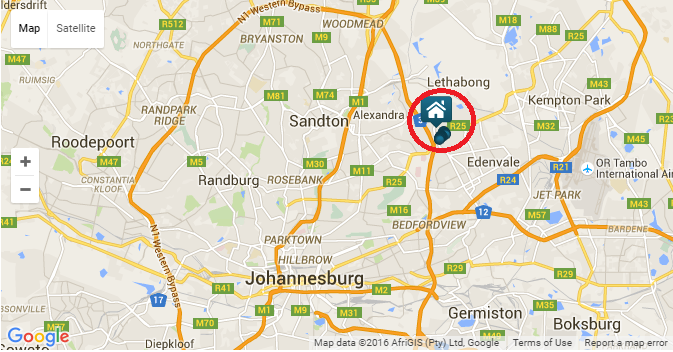
\includegraphics[width=0.75\textwidth]{images/offices_map.PNG}
\vskip10pt
\caption[Map showing potential office location in Longmeadow, north of Johannesburg]{Map showing potential office location in Longmeadow, north of Johannesburg}
\label{fig:map}
\end{figure}

\begin{figure}[H]
\centering
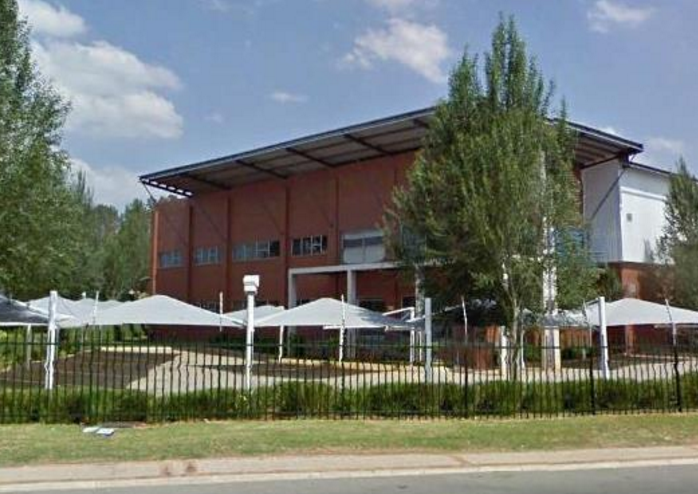
\includegraphics[width=0.55\textwidth]{images/offices_building.PNG}
\vskip10pt
\caption[Potential offices for Uvuka that are available and suit our current business size with room for expansion]{Potential offices for Uvuka that are available and suit our current business size with room for expansion}
\label{fig:offices}
\end{figure}

\section{Production and manufacturing}
\textit{Ben do this bit :P Talk about how we will make the parts elsewhere, and then assemble it ourselves or whatever we are doing, also about how making it in-house will improve quality control and allow us to change things quicker than if we had to go through a whole supply chain, that kind of thing.}
%include risk management stuff associated with manufacturing here?

\section{Staff and team expansion}
\textit{Gareth, write here about the team and the sales person you wanted to hire, and possibly firing Ben.}

\section{Future developments}
%Munawwar/Luke add your bit here from the poster or slideshow, go wild.
In the future, Uvuka will seek to become a automotive safety company by expanding the product range. This will comprise of four stages:
\begin{enumerate}
\item Immediate implementation (year 5)
\item Short-term (year 10)
\item Intermediate
\item Long-term
\end{enumerate}

\subsection{Immediate Implementation}
After the 5 year mark, we as a company will have started diversifying our products to suit more road users, from private family use to large freight companies. We will continue in this way for a few more years, strengthening our reputation and position in the market as a road safety company. We intend to expand up into Southern Africa and capitalise on the emerging markets on our doorstep.

%TODO - add more detail for the technical description of some of these features perhaps.
In terms of the physical additions to our device, the following provide some insight into the possibilities:
\begin{itemize}
\item \textit{Insurance feature:} An added road-facing camera integrated into the device, recording footage which could be used in the event of an accident to prove driver innocence.

\item \textit{Vehicle tracking and monitoring:} GPS and inertial measurement sensors integrated into the device will allow a fleet manager to monitor the company vehicles.

\item \textit{Smart phone application:} Linking the device via GSM/Bluetooth/Wi-Fi could allow easier access to a history of driving activity.
\end{itemize}

\subsection{Short-Term Expansion}
After 10 years, we aim to partner with various car manufacturers and integrate our camera systems into their vehicles, much like the current Toyota and Lexus cars that have similar drowsiness detection systems \cite{lexus} \cite{toyota}. We will aim to assist the car manufacturers we join to incorporate additional warning levels such as independent brake control to either jolt the driver awake or stop the car completely, depending on if the driver reacts to the previous warnings.

\subsection{Intermediate Expansion}
New technology will run concurrently with the short-term expansion goals to control a driver's cellphone notification alerts, vehicle radio, and any other additional stimuli. This will seek to reduce the distractions faced by the driver. Research into how drivers react to disturbances while driving will need to be undertaken in order to ensure the product meets its objectives.

\subsection{Long-Term Expansion}
In the not-too-distant future, the road will be filled with self-driving vehicles. This will make our current Uvuka Pro device redundant as drivers will not necessarily need need to be kept awake at the wheel. However, the inevitable transition period ahead will require drivers to be on alert in the event that the autonomous system is unable to navigate the vehicle. If our system detects that the occupant is not fast asleep or too drowsy to drive, warnings could be sounded and the occupant alerted to the fact that they need to take over from the automated system. Similarly, the cabin camera can be reconfigured to send signals to the car to indicate whether the occupants are awake or asleep, and adjust the driving style accordingly.

\begin{appendices}
\appendix
\chapter{Insert Here}
\label{app:Insert Here}	
\newpage

\chapter{Another}
\label{app:Another}
\end{appendices}	%for use with appendices
\newpage
\renewcommand\bibname{References}
\bibliography{Aldera_bibliography}
\bibliographystyle{ieeetr}
%changing this to ^ieeetran^ and downloading the zip and compiling on Rob's PC will produce a reference list that has the URLs in it, don't worry about this for now.
\addcontentsline{toc}{chapter}{References}

\newpage	%this keeps the header/footer working on the last page. Do not type anything after this.

\end{onehalfspace}
\end{document}

%-------------------------------Figures--------------------------------%
\begin{figure}[H]
\centering
\includegraphics[width=0.4\textwidth]{images/%}
\vskip10pt
\caption[The caption that appears in the list of figures]{The caption that appears under the figure}
\label{fig:exam}
\end{figure}

\begin{figure}[H]
\centering
\begin{subfigure}[t]{0.49\textwidth}
\centering
\includegraphics[width=0.9\linewidth]{images/%}
\caption{This is figure a}
\label{fig:figureA}
\end{subfigure}
\begin{subfigure}[t]{0.49\textwidth}
\centering
\includegraphics[width=0.9\linewidth]{images/%}
\caption{This is figure b}
\label{fig:figureB}
\end{subfigure}
\caption{Caption}
\end{figure}

\begin{wrapfigure}{r}{0.5\textwidth}
\begin{center}
\includegraphics[width=0.48\textwidth]{images/ %}
\end{center}
\caption{A gull}
\end{wrapfigure}

As can be seen in \cref{fig:exam}\\
%-------------------------------Headings-------------------------------%
\chapter{Chapter Title}
\label{ch:Chapter Title}

\section{Section Title}
\label{sec:Section Title}

\subsection{Subsection Title}
\label{subsec:Subsection Title}

\subsubsection{Subsubsection Title}
\label{bb:Subsubsection Title}
%---------------------------Tables and Lists---------------------------%
\renewcommand{\contentsname}{Table of Contents} %change table of contents's name from 'contents' to 'table of contents'
\newpage %page break
\phantomsection %for some reason this gets the bookmarks to work

\tableofcontents



%\addcontentsline{toc}{chapter}{Section:} %add "table of contents" to the table of contents
\newpage %page break
\input{\filepath /list_of_figures.tex}
\input{\filepath /list_of_tables.tex}
\input{\filepath /list_of_example.tex}

\startcontents[chapters] %mini table of contents
\printcontents[chapters]{}{1}{}
\newpage
%-----------------------------Insert Pages-----------------------------%
\includepdf[pages={1}]{ %filename.pdf}
%-------------------------------Appendix-------------------------------%
\startcontents[section]
\printcontents[section]{}{1}{}
\newpage
\addcontentsline{toc}{section}{1. %}
%--------------------------------Citing--------------------------------%
\footnote{\cite{aa}}
\cite{aa,bb}
%--------------------------Custom Bibliography-------------------------%
makebst
%----------------------------Maths & Symbols---------------------------%
http://www.artofproblemsolving.com/Wiki/index.php/LaTeX:Symbols
http://www.tex.ac.uk/tex-archive/info/symbols/comprehensive/symbols-a4.pdf
$Hardcore \: maths \: here \: \therefore \ddot{\theta}^{2} = \left(\dfrac{\omega_{n}}{17a}\right) \times 9$
$$ More \: maths: \sqrt{52} + F_{1} = 6 \times 10^{5} \: Hz$$
$\mathrm{\today}$ %maths in normal font
%---------------------------Lines and Spacing--------------------------%
\noindent\makebox[\linewidth]{\rule{\textwidth}{0.4pt}}
\vspace{11pt}
\hspace{-11pt}
\hphantom{11pt}
%----------------------------Page Numbering----------------------------%
\pagenumbering{gobble} %remove page numbering
\pagenumbering{roman} %roman letters page numbering
\pagenumbering{arabic} %arabic letters page numbering
\setcounter{page}{1} %reset page numbers
%--------------------------------Tables--------------------------------%
\begin{table}[H]
\caption{Caption of table}
\addvbuffer[12pt 8pt]{
\begin{tabularx}{0.3\textwidth}{@{}rcl@{}}
\hline
\multicolumn{3}{@{}c@{}}{\textbf{Title}}\\
\hline
Info	& 3	& mm\\
Item	& 5	& x $\approx$ 34\\
\cline{2-2}
Width	& 4	& miles\\
Depth	& 7	& \pbox{20cm}{This is the first \\ cell}\\
\hline
\label{tab:capt}
\end{tabularx}
}
\end{table}

\begin{tabularx}{\textwidth}{@{}lX@{}}
 & \\
\end{tabularx}

\\
\\
\begin{tabular}{ l l }
 & \\
\end{tabular}
%--------------------------------Lists---------------------------------%
http://en.wikibooks.org/wiki/LaTeX/List_Structures

%TC:ignore
\begin{itemize} \itemsep1pt \parskip0pt \parsep0pt \vspace{-6pt}
%TC:endignore
\item[-] The first item
\item[-] The second item
\item[-] The third etc \ldots
\end{itemize}

\begin{enumerate} [label=\bfseries Exercise \arabic*:]
\item The first item
\item The second item
\item The third etc \ldots
\end{enumerate}

\begin{description}
\item[First] The first item
\item[Second] The second item
\item[Third] The third etc \ldots
\end{description}

\begin{description}
\item[First] \hfill \\
The first item
\item[Second] \hfill \\
The second item
\item[Third] \hfill \\
The third etc \ldots
\end{description}

Inline lists are \begin{enumerate*}[label=\itshape\alph*\upshape)]
\item formatted within their paragraph;
\item usually labelled with letters; and
\item usually have the final item prefixed with
`and' or `or',
\end{enumerate*} like this example.

\example{Your first example}
\label{1st_ex}
\example{Your second example}
\label{2nd_ex}
\example{Your third example. (See example \ref{1st_ex} and \ref{2nd_ex})}
%----------------------------------------------------------------------%
\fi